\documentclass{whutmod}
\usepackage{metalogo}
\usepackage{float}
\usepackage{subfigure} 
\usepackage{url}
\usepackage{booktabs}
\usepackage[style=caspervector,backend=biber,utf8]{biblatex}
\addbibresource{wenxian.bib}
\team{23}
\membera{刘子川}
\joba{编程}
\memberb{程宇}
\jobb{建模}
\memberc{陈荣兴}
\jobc{建模}
\hypersetup{
	colorlinks=true,
	linkcolor=black
}

\title{基于因子分析与灰色关联分析对武汉市人才吸引力的量化评价}
\tihao{4} 

\begin{document}

	%\maketitle
	
	\begin{abstract}

城市的发展对人才的吸引力两者之间是相互联系与制约的,因此需要政府决策与措施影响,使城市增强对人才的吸引力。本文结合武汉的发展特点,利用\textbf{爬取}后的数据较全面的选择合适的指标进,通过\textbf{因子分析}的方法为武汉市不同年份人才吸引力打分;再对人才进行产业类别分类,通过\textbf{灰色关联分析}筛选出合适的因子后再横向比较各城市综合得分,并结合当地人才政策评价对人才吸引力的水平提出合理化建议。
~\\%~\\为换行

针对问题一,通过\textbf{因子分析模型}分析武汉2013—2017年相关数据,对武汉各年的人才吸引力进行\textbf{量化打分}。本组首先根据题目要求和以往人才吸引要素研究,确立要素框架并\textbf{爬取}合适的人才吸引力因素。在标准化数据通过\textbf{KMO检验}后,利用SPSS对各个因素进行\textbf{主成分分析}以确定公因子数目,求解旋转后因子荷载矩阵并对公因子命名,计算武汉各年人才吸引力综合得分。综合得分结果为\textbf{-77.99、-30.08、-11.90、42.35、77.63}。综合得分表明武汉2013—2017人才吸引力逐年上升,且2015—2016年上升幅度最大,与城市实际发展情况相符合。
~\\

针对问题二,本文在问题一模型的基础上进行改进,将人才分为第一、第二和第三产业人才并用\textbf{灰色关联分析}筛选出每类人才相应的人才吸引力因素。然后将筛选后的数据用SPSS进行\textbf{因子分析}得到成都、天津、西安、南京和武汉2013—2017年的三类人才吸引力因子分析模型,并计算每个城市各年针对三类人才的人才吸引力\textbf{综合得分}。横向比较各个城市的综合得分,相较与其他城市,武汉市近几年对第二、三产业人才的吸引力有较高水平,相对于西安和成都,武汉市具有较强的人才吸引力,符合地区的经济发展特点。
~\\

针对问题三,基于问题一中的武汉市人才吸引力评价模型以及人才政策对人才吸引力的量化评价,并结合问题二中武汉相较于其他四个同类城市在人才吸引力上的优势与不足,给武汉市人力资源管理部门的领导写一篇建议报告。
~\\

本文中所提到的模型优点主要有两点:一、选取的指标从多维度、全方面考虑,收集的数据真实可靠;二、利用灰色关联度筛选出三类人才的人才吸引力要素,相较于人工选取指标具有客观性、严谨性。
  
\keywords{因子分析模型\quad  主成分分析\quad  灰色关联分析\quad 数据库爬虫\quad }
		
	\end{abstract}
	
	%目录
	\tableofcontents
	\newpage	%换页符
	
	\section{问题重述}	
	\subsection{问题背景}
现代管理中,彼得德鲁克提出了"人力资源"的概念并认为"人力资源是与其他资源不一样的特殊资源",人力资源的其中一个特质是其具有自主流动性。根据勒温的场论,人才会根据自身需求与环境的适应性而做出离开或者留在某个环境的决定。人才是一个城市保持竞争活力和创新力的关键,在世界各国和全国各地积极推出人才吸引的政策背景下,一个地区的人才吸引力的核心内涵就是这个地区所具有的可以影响人才选择的能力。

全面、科学、系统地评价一个城市的人才吸引力是制定人才吸引计划的前提,城市人才吸引评价指标的选取受多方面影响,关键是要符合人才的理想,满足人才的需求和愿望。按照重要程度,人才的需求可以分为发展前景,收入和环境。发展前景是首要关心的因素,收入是人才流动的另一关键因素,环境因素包括治安、交通、污染、教育、医疗、购物等,也都是会考虑的因素。




	
	\subsection{问题提出}
围绕城市地区人才吸引力水平,以城市多指标评价体系为依据,依次提出以下问题:
		 
	\begin{itemize}
	\item [(1)] 根据数学模型及收集的数据,定量地分析武汉市的人才吸引力水平,并就武汉市的人才政策对人才吸引力水平的影响作出定量评价。
	\item [(2)] 结合人才类别,针对不同类型的人才,深入分析比较武汉市与其他同类城市在人才吸引力上的优势与不足,并给出有效提升人才吸引力的可行方案。
	\item [(3)] 结合模型结果及分析,给武汉市人力资源管理部分写一篇建议报告,要求论点明确,论据充分。
	\end{itemize}
	
	\section{模型假设}
	\begin{itemize}
		\item [(1)] 假设相同的行业在不同的城市里吸引力影响因素相同,每个行业在不同城市里的发展模式近似相同。


		\item [(2)] 人才会考虑未来一段时间内自身对于发展前景、收入、环境的需求的变化。
	\item [(3)] 政策对人才吸引力的影响转换成三个影响因素——地方财政支出与收入和固定资产投资总额。
		\item [(4)] 人才的迁移是在追求效用最大化,人才的行为仅受到城市因子的影响,忽略人的非理性行为。
	\end{itemize}
	
	
	\section{符号说明}
%	每行都有线的表
%	\begin{center}
%		\begin{tabular}{cc}
%			\hline
%			\makebox[0.3\textwidth][c]{符号}	&  \makebox[0.4\textwidth][c]{意义} \\ \hline
%			$C_{0}$	    &  污染源初始浓度 \\ \hline
%			$C(x,t)$	    &  污染浓度随时空变化 \\ \hline
%			$u_{x}$	    &  江河平均纵向流速 \\ \hline
%			$E_{x}$  &  铊在江河纵向弥散系数\\ \hline
%		$p$   &  面污染物纵向距离\\ \hline
%			$K_{c}$	    & 污染物降解系数  \\ \hline
%		    $a$	& 污染超标系数 \\ \hline
%		     $x$	& 距污染源的一维距离 \\ \hline
%		      $t$	& 距污染发生后的时间 \\ \hline
%		       $V_{A}$	& 溶液摩尔体积 \\ \hline
%		      $M_{B}$	& 江水的摩尔质量 \\ \hline
%		     $\mu_{B}$	& 溶剂的粘度 \\ \hline		      
%		\end{tabular}
%	\end{center}

%三线表
	\begin{table}[H]
	\label{biao} \centering
		\begin{tabular}{cc}
			\toprule[1.5pt]
			\multicolumn{1}{m{5cm}}{\centering 符号} & \multicolumn{1}{m{5cm}}{\centering 说明} \\
			\midrule[1pt]
			$F$	 &  城市各年人才吸引力综合得分  \\ 
			$F_{1}$ &  工业发展与薪酬因子 \\ 
			$F_{2}$	 &  医疗卫生环境因子 \\ 
			$F_{3}$  &  经济贸易因子 \\ 
			$F_{4}$  &  拥挤程度因子 \\ 
			$X$  &  原始指标 \\ 
			$\overline{X}$  &  指标平均值 \\ 
			$\widetilde{X}$  &  同向化指标 \\ 
	     	$\delta_{X}$  &  指标标准差 \\ 
	     	$Z$  & 标准化指标 \\ 
	     	$R$  & 相关系数矩阵 \\ 
	     	$\lambda_{p}$  & 相关系数矩阵特征值 \\ 
	     	$\eta _ {p}$  & 标准正交化特征向量 \\ 
	     	$\Lambda$ & 因子载荷矩阵 \\ 
	     	$\sigma_{i}$ & 方差 \\
	     	$\alpha_{i j}$ & 载荷因子 \\
	     	$k$ & 两极最小差 \\
	     	$K$ & 两极最大差 \\
	     	$\Delta _{i}(t)$ & 特征序列与因素序列的序列差 \\
			\bottomrule[1.5pt]
		\end{tabular}
	\end{table}

	\section{问题一模型的建立与求解}
	\subsection{问题的描述与分析}

	针对问题一,本题要求对武汉的人才吸引力做出量化评价。对于人才吸引力水平模型,现在主要存在的问题是定性研究较多、量化评价较少,对变量之间的关系讨论更是不足。本文采用因子分析法建立模型,将通过不同的因子对变量的影响程度进行分析,建立客观评价模型。首先根据题目要求和以往人才吸引要素研究,寻找合适的人才吸引力因素,确立要素框架并爬取各个因素相对应的数据。在将所得数据进行无量纲化处理后,进行$KMO$检验和巴特利特检验以验证所选变量是否适合做因子分析。通过主成分分析法确定公因子数目,求解旋转后因子荷载矩阵并对公因子命名,最后利用因子得分与其奉献率计算武汉各年人才吸引力综合得分,其流程图如图~\ref{llll}~所示:


	\begin{figure}[H]
		\centering
		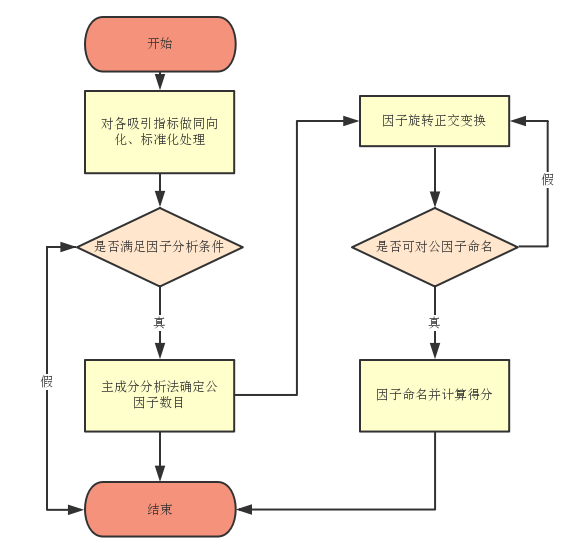
\includegraphics[width=\textwidth]{figures/1111.png}
		\caption{因子分析算法流程图}\label{llll}
	\end{figure}

		\subsection{预备工作}
		\subsubsection{评价指标体系构建}
		参考国家统计局对人才标准的划分,此处对人才的界 定是指,具有大专及以上学历的人员,以及具有初级以上 专业技术职称的人员或在专业技术岗位上工作的人员。
		
		在构建武汉市人才吸引力评价指标体系时,在指标方面,若选取总量太多,在评价模型时太为复杂,可行性低,若数据太少则评价不够准确,脱离实际性。因此为尽可能客观反映吸引力,我们在遵循建立指标体系的科学性、系统性、可操作性、可比性原则\parencite{lepawsky2010metropolis},并兼顾总量指标和相对指标,选取城市发展前景、主要行业收入、政府影响、环境因素、年末总人口共5个二级指标和33个三级指标,多维度、全方面的考虑各个指标对人才吸引力的影响。具体指标体系如图~\ref{lct}~所示: 	
		\begin{figure}[H]
			\centering
			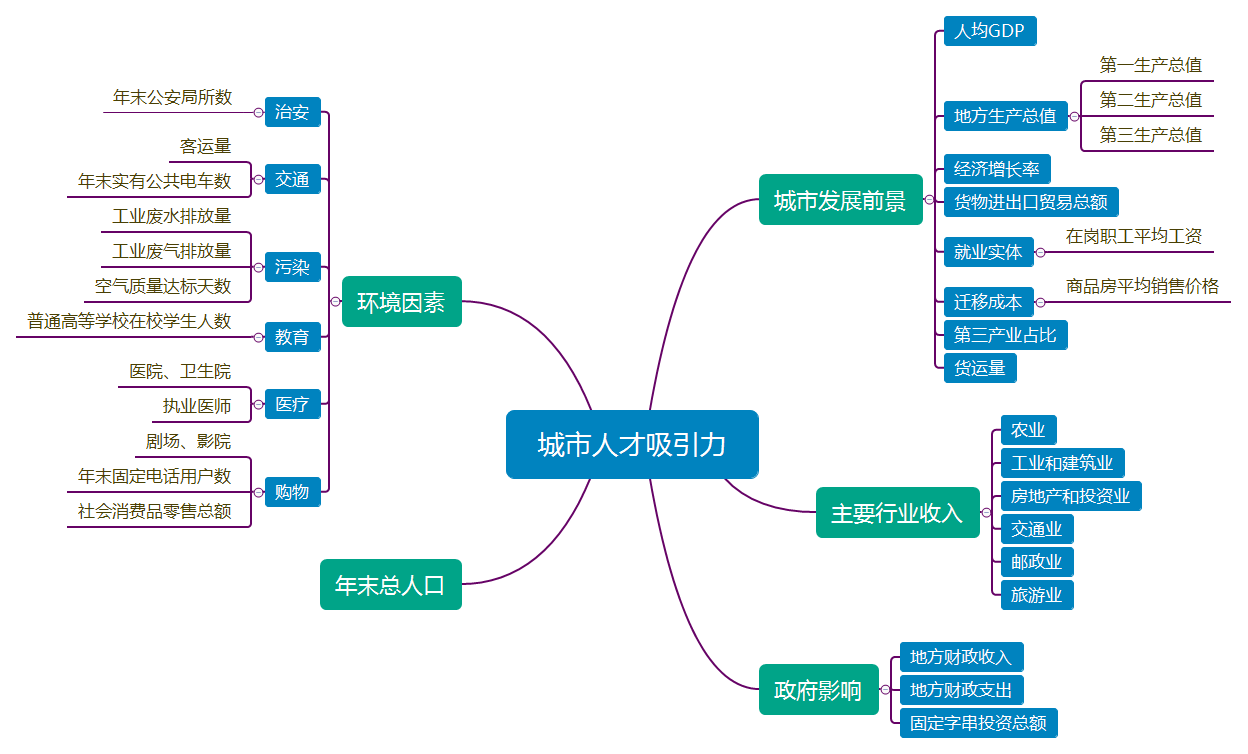
\includegraphics[width=\textwidth]{figures/clt.png}
			\caption{城市人才吸引力指标体系}\label{lct}
		\end{figure}  
		
		\subsubsection{同向化处理}

		在评价城市人才的指标中,工业废水废气排放量和商品房平均销售价格不越高越好,为方便比较,对这三个指标进行同向化处理\parencite{张瑞红2012河南省产业集群环境人才吸引力评价研究}, 其公式如下:
		\begin{gather}
		\widetilde{X}=-(X-\overline{X})
		\end{gather}
		式中:$X$原始指标,$\overline{X}$为原始指标$X$的平均值,$\widetilde{X}$为同向化指标。
		
		\subsubsection{标准化处理}
		为了对变量进行比较并消除由于观测量纲的差异及数量级差异所造成的影响,将样本观测数据进行标准化处理,使标准化的变量均值为$0$,方差为$1$。其处理方法如下:
		\begin{gather}
		Z=\frac{X-\overline{X}}{\delta_{X}}
		\end{gather}
		式中:$\overline{X}$为$X$的均值,$\delta_{X}$是$X$的标准差。
		
		\subsubsection{KMO与Bartlett检验}
		根据标准化处理后的指标数据,利用$SPSS23.0$统计软件进行$KMO$和巴特利特检验,以确认所选变量是否适合做因子分析,结果如表\label{tab1}所示:
		% Table generated by Excel2LaTeX from sheet 'Sheet1'
		\begin{table}[H]
			\centering
			\caption{KMO和Bartlett的检验}\label{tab1}
			\begin{tabular}{cc|cc|cc}
				\toprule[1.5pt]
				\multicolumn{4}{c|}{取样足够度的Kaiser-Meyer-Olkin度量} & \multicolumn{2}{c}{0.859} \\
				\midrule
				\multicolumn{2}{c|}{\multirow{3}[2]{*}{Bartlett的球形度检验}} & \multicolumn{2}{c|}{近似卡方} & \multicolumn{2}{c}{1183.981} \\
				\multicolumn{2}{c|}{} & \multicolumn{2}{c|}{df} & \multicolumn{2}{c}{78} \\
				\multicolumn{2}{c|}{} & \multicolumn{2}{c|}{Sig.} & \multicolumn{2}{c}{.000} \\
				\bottomrule[2pt]
			\end{tabular}%
			\label{tab:addlabel}%
		\end{table}%
		
		由上表可知,巴特利特球度检验统计量的观测值为$1183.981$,相应的概率$P$值接近$0$。若显著性水平$α$为$0.5$,概率$P$小于显著性水平$α$,应拒绝零假设,认为相关系数矩阵与单位阵有显著差异,即因子协方差矩阵不是单位阵。同时,$KMO$值为$0.859$,$KMO>0.8$,根据$KMO$ 度量标准可知原有变量适合进行因子分析。
		
		
		

	\subsection{模型的建立与求解}
	\subsubsection{公因子的确定}
	根据上述指标标准化后,其对应相关系数矩阵部分数据见表~\ref{shuju2}~所示(详见附录):
	%三线表
	\begin{table}[H]
		 \centering
		\caption{相关系数矩阵部分数据}\label{shuju2}
		\begin{tabular}{ccccccc}
			\toprule[2pt]
			\multicolumn{1}{m{1cm}}{\centering } &
			\multicolumn{1}{m{2cm}}{\centering $X_{1}$} & \multicolumn{1}{m{2cm}}{\centering $X_{2}$} & \multicolumn{1}{m{2cm}}{\centering $X_{3}$}&
			\multicolumn{1}{m{2cm}}{\centering $X_{4}$}&
			\multicolumn{1}{m{1cm}}{\centering ........} &
			\multicolumn{1}{m{2cm}}{\centering $X_{33}$}
			\\
				\midrule[1pt]
			$X_{1}$&1.000	 &  0.727 & -0.423&0.967&........& -0.928\\ 
			$X_{2}$& &  1.000 & -0.796&0.822&........&-0.814\\ 
			$X_{3}$& &   & 1.000&-0.620&........&0.682\\ 
			$X_{4}$& &   & &1.000&........&-0.955\\ 
			........& &   & & &........&........\\ 
			$X_{33}$& &   & & &........&1.000\\
			\bottomrule[2pt]
		\end{tabular}
	\end{table}
	
	设$\lambda_{1} \geqslant \lambda_{2} \geqslant \cdots \geqslant \lambda_{p}$为样本相关系数矩阵$R$的特征值,$\eta _ { 1 } , \eta _ { 2 } , \cdots , n _ { p }$为相应的标准正交化特征向量。设$m<p$,则因子载荷矩阵$\Lambda$为:
	\begin{gather}
	\Lambda=\left[\sqrt{\lambda_{1}} \eta_{1}, \sqrt{\lambda_{2}} \eta_{2}, \cdots, \sqrt{\lambda_{m}} \eta_{m}\right]
	\end{gather}
    用$\boldsymbol{R}-\boldsymbol{\Lambda} \boldsymbol{\Lambda}^{\mathrm{T}}$对角元来估计特殊因子的的方差:
	\begin{gather}
	\sigma_{i}^{2}=1-\sum_{j=1}^{m} \alpha_{i j}^{2}
	\end{gather}
	式中:$\sigma_{i}$为方差,$\alpha_{ij}$表示载荷因子。由上述分析,得总方差解释部分数据如表~\ref{biaosan}~所示:	
		\begin{table}[H]
		\centering
		\caption{总方差解释}\label{biaosan}
		\begin{tabular}{ccccccc}
			\toprule[1.5pt]
		\multicolumn{1}{m{1cm}}{\centering } &
				\multicolumn{1}{m{1.5cm}}{\centering  } &
		 \multicolumn{1}{m{3cm}}{\centering 初始特征值} &
		 		\multicolumn{1}{m{1cm}|}{\centering  } &
		\multicolumn{1}{m{1cm}}{\centering  } &
		 \multicolumn{1}{m{3cm}}{\centering 提取载荷平方和}&
		 		\multicolumn{1}{m{1.5cm}}{\centering  } \\\hline
		\multicolumn{1}{m{1cm}|}{\centering  成分} &
		\multicolumn{1}{m{1.5cm}}{\centering  总计} &
		\multicolumn{1}{m{3cm}}{\centering  方差百分比} &
		\multicolumn{1}{m{1cm}|}{\centering  累积} &
		\multicolumn{1}{m{1cm}}{\centering  总计} &
		\multicolumn{1}{m{3cm}}{\centering  方差百分比} &				\multicolumn{1}{m{1.5cm}}{\centering  累积} \\

			\midrule[1pt]
			1&25.330&76.758&76.758&25.330&76.758&76.758 \\
			2&4.025&12.197&88.956&4.025&12.197&88.956 \\
			3&2.373&7.191&96.147&2.373&7.191&96.147 \\
			4&1.271&3.852&99.920&1.271&3.852&99.920 \\
			5&5.129e-15&1.554e-14&100.0&&& \\
			6&1.330e-15&4.031e-15&100.0&&& \\
			7&6.062e-16&1.837e-15&100.0&&& \\
			8&5.067e-16&1.535e-15&100.0&&& \\
			9&4.532e-16&1.373e-15&100.0&&& \\
			10&3.335e-16&1.011e-15&100.0&&& \\
			11&3.137e-16&9.506e-16&100.0&&& \\
			12&2.585e-16&7.834e-16&100.0&&& \\
			13&1.990e-16&6.031e-16&100.0&&& \\
			......&......&.......&100.0&&& \\
			......&......&.......&100.0&&& \\
			33&-2.279e-15&-6.908e-15&100.0&&& \\
			\bottomrule[1.5pt]
		\end{tabular}
	\end{table}
	
	
	由表~\ref{biaosan}~特征根知,因子$F_{1}$的特征值$\lambda_{1}=25.330$,占方差的 $76.75\%$。由碎石图~\ref{123}~可知,当提取$1,2$个公因子时,特征值变化非常明显,当提取第$5$个以后的公因子时,特征值变化比较小,基本趋于平缓。由此说明,提取$4$个公因子对原变量信息的刻画有显著作用。因此,在这里我们提取$4$个公共因子,这$4$个公因子的累计方差达到$99.92\%$,即这$4$个公因子可以反映原来$33$个指标的$99.92\%$的信息量,可见采用前\textbf{4个公因子}对武汉2013—2017年人才吸引力进行评价是比较合适的。
	
	\begin{figure}[H]
		\centering
		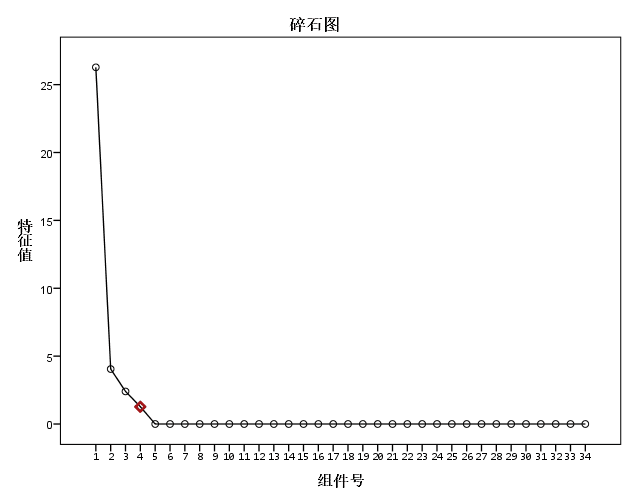
\includegraphics[width=\textwidth]{figures/123.png}
		\caption{碎石图}\label{123}
	\end{figure} 
	
	\subsubsection{因子命名与载荷矩阵计算}

	表~\ref{cehngfenjuzheng}~是初始因子载荷矩阵(详见附录),由此可写出因子分析模型的如下:
	\begin{gather}
	\begin{array} { l } { \mathrm { X } _ { 1 } = 0.989 \mathrm { F } _ { 1 } + 0.123 \mathrm { F } _ { 2 } - 0.074 \mathrm { F } _ { 3 } - 0.031 \mathrm { F } _ { 4 } } \\ { \mathrm { X } _ { 2 } = 0.795 \mathrm { F } _ { 1 } - 0.556 \mathrm { F } _ { 2 } - 0.193 \mathrm { F } _ { 3 } - 0.151 \mathrm { F } _ { 4 } } \\ { \ldots \ldots } \\ { \mathrm { X } _ { 33 } = - 0.958 \mathrm { F } _ { 1 } + 0.176 \mathrm { F } _ { 2 } - 0.060 \mathrm { F } _ { 3 } + 0.220 \mathrm { F } _ { 4 } } \end{array}
	\end{gather}
			\begin{table}[H]
	\centering
	\caption{初始因子载荷矩阵}\label{cehngfenjuzheng}
	\begin{tabular}{ccccc}
		\toprule[2pt]
		\multicolumn{1}{m{2cm}}{\centering 指标} &
		\multicolumn{1}{m{1cm}}{\centering $F_{1}$} & \multicolumn{1}{m{1cm}}{\centering $F_{2}$} & \multicolumn{1}{m{1cm}}{\centering $F_{3}$}&
		\multicolumn{1}{m{1cm}}{\centering $F_{4}$}\\
		\midrule[1pt]
		地方财政预算支出&0.989	 & 0.123 & -0.074&-0.031\\ 
		固定资产总额&0.795 &-0.556 &-0.193&0.151\\ 
		年末邮政局数&-0.548 &0.768  &-0.333&0.008\\ 
		执业医师人数&0.994 &-0.027 &-0.245 &0.002\\ 
		........& ........&  ........ &........ &........ \\ 
		年末固定电话数&-0.958 &-0.176   &-0.060 &0.220 \\
		\bottomrule[2pt]
	\end{tabular}
\end{table}
		表~\ref{cehngfenjuzheng}~中的每个数据表示了相应因子变量对相应原变量的相对重要程度。由于得到的公共因子与各指标的载荷分布归类比较困难,需要对因子载荷矩阵进行正交旋转,这里运用方差最大正交旋转法\parencite{宋鸿2010城市人才吸引力的影响因素及提升对策},得到旋转后的因子载荷矩阵表~\ref{xuanzhuanhuo}~所示(详见附录):
			\begin{table}[H]
			\centering
			\caption{旋转后的因子载荷矩阵}\label{xuanzhuanhuo}
			\begin{tabular}{ccccc}
				\toprule[2pt]
				\multicolumn{1}{m{2cm}}{\centering 指标} &
				\multicolumn{1}{m{1cm}}{\centering $F_{1}$} & \multicolumn{1}{m{1cm}}{\centering $F_{2}$} & \multicolumn{1}{m{1cm}}{\centering $F_{3}$}&
				\multicolumn{1}{m{1cm}}{\centering $F_{4}$}\\
				\midrule[1pt]
				地方财政预算支出&0.870	 & 0.356 & 0.076&0.331\\ 
				固定资产总额&0.469 & 0.311 &0.678&0.473\\ 
				年末邮政局数&-0.291 & -0.390  &-0.867&0.105\\ 
				执业医师人数&0.787 &0.496   &0.259 &0.259\\ 
				........& ........&  ........ &........ &........ \\ 
				年末固定电话数&-0.872 &-0.277   &-0.384 &-0.124 \\
				\bottomrule[2pt]
			\end{tabular}
		\end{table}
	
	根据表~\ref{xuanzhuanhuo}~发现,旋转在\textbf{9次迭代}后已收敛。旋转后的因子系数已经明显向两极分化,有了更鲜明的实际意义。因子载荷的绝对值越大,则表明该因子与变量的重叠性越高,在解释因子的时候就越重要。

		第一因子$F_{1}$主要包含地区生产总值、第一第二产业生产总值、在岗职工平均工资和人均GDP等,这些指标包含了地区工业发展水平以及人均薪酬水平故将其命名为\textbf{工业发展与薪酬因子}。第二因子$F_{2}$主要包含持证医师人数,医院卫生院个数以及一年内空气质量达到及好于二级的天数等,这些指标包含了地区医疗卫生水平和居民生活环境,故将其命名为\textbf{医疗卫生环境因子}。第三因子$F_{3}$主要包含固定资产投资总额与货物进出口总额,该指标反映了城市贸易与经济发展水平,故将其命名为\textbf{经济贸易因子}。第四因子$F_{4}$包含年末总人口与旅游生产总值,反映了城市人口与拥挤程度故将其命名人口与\textbf{拥挤程度因子}。

	\subsubsection{求得因子得分和综合绩效得分}
	采用回归法估计因子得分系数,并输出因子得分系数矩阵,其结果见表~\ref{defenyinzi}~所示(详见附录):
				\begin{table}[H]
		\centering
		\caption{成分得分系数矩阵}\label{defenyinzi}
		\begin{tabular}{ccccc}
			\toprule[2pt]
			\multicolumn{1}{m{2cm}}{\centering 指标} &
			\multicolumn{1}{m{1cm}}{\centering $F_{1}$} & \multicolumn{1}{m{1cm}}{\centering $F_{2}$} & \multicolumn{1}{m{1cm}}{\centering $F_{3}$}&
			\multicolumn{1}{m{1cm}}{\centering $F_{4}$}\\
			\midrule[1pt]
			地方财政预算支出&0.052 & -0.017 & -0.021&0.024\\ 
			固定资产总额&-0.063 & 0.045 &0.127&0.137\\ 
			年末邮政局数&0.022 &-0.079  &-0.195&0.109\\ 
			执业医师人数&0.007 &0.064 &0.021 &0.009\\ 
			........& ........&  ........ &........ &........ \\ 
			年末固定电话数&-0.109 &0.093 &-0.068 &0.094 \\
			\bottomrule[2pt]
		\end{tabular}
	\end{table}
	则根据表~\ref{defenyinzi}~可以计算出四个主因子得分,表达式分别为:
	\begin{gather}
	\begin{matrix}
	F_{1}=0.052x_{1}-0.063x_{2}+0.022x_{3}+0.007x_{4}+\cdots-0.109x_{33}\hfill\\ 
	F_{2}=-0.017x_{1}+0.045x_{2}-0.079x_{3}+0.064x_{4}+\cdots+0.093x_{33}\hfill\\ 
	F_{3}=-0.021x_{1}+0.127x_{2}-0.195x_{3}+0.021x_{4}+\cdots-0.068x_{33}\hfill\\ 
	F_{4}=0.024x_{1}+0.137x_{2}+0.109x_{3}+0.009x_{4}+\cdots+0.094x_{33}\hfill
	\end{matrix}
	\end{gather}
	
	利用SPSS软件计算得到旋转后的因子贡献及贡献率如表~\ref{fff}~所示:
			\begin{table}[H]
	\centering
	\caption{旋转后因子贡献及贡献率}\label{fff}
	\begin{tabular}{cccc}
		\toprule[2pt]
		\multicolumn{1}{m{2cm}}{\centering 因子}&
		\multicolumn{1}{m{2cm}}{\centering 贡献} & \multicolumn{1}{m{2cm}}{\centering 贡献率} & \multicolumn{1}{m{2cm}}{\centering 累计}\\
		\midrule[1pt]
		$F_{1}$	 &  18.238 & 55.267&55.267\\ 
		$F_{2}$ &  5.889 & 17.845&73.112\\ 
		$F_{3}$	 &  4.826 &14.623&87.735\\ 
		$F_{4}$  &  40.470& 12.265&99.920\\ 
		\bottomrule[2pt]
	\end{tabular}
\end{table}
	
	由此计算出的因子得分,可以量化描述城市人才吸引力水平,利用因子得分可以从不同角度对城市人才吸引力水平进行比较分析。为了便于对各城市进行人才吸引力评价,现利用武汉每年的因子得分表计算综合得分,吸引力水平的获取是基于总方差分解表中旋转后各因子的方差贡献率及计算所得的城市各因子得分获取的。其计算公式如下:
	\begin{gather}
	\mathrm { F } = \left( 55.267 \mathrm { F } _ { 1 } + 17.845 \mathrm { F } _ { 2 } + 14.623 \mathrm { F } _ { 3 } + 12.265 \mathrm { F } _ { 4 } \right) / 99.92
	\end{gather}
	经计算,纵向比较武汉每年的综合因子得分后绘制直方图:
		\begin{figure}[H]
		\centering
		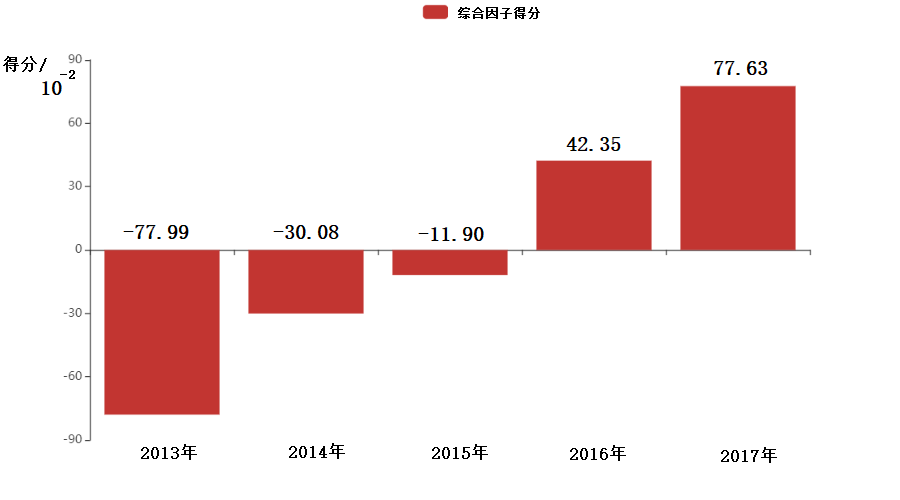
\includegraphics[width=\textwidth]{figures/wuhan.png}
		\caption{综合因子得分}
	\end{figure} 
	\subsection{结果分析}

	(1)人才吸引力的33个指标经因子分析和主成分分析后综合成的4个公因子,由回归法求得的图~\ref{defenyinzi}~、~\ref{fff}~所示,4个公因子的累计方差达到99.92\%,反应的信息量达到比较合适的比例。
	
	(2)根据武汉每年的因子得分表计算构建出的2013-2017年武汉综合因子得分表表明武汉市对于人才吸引力水平整体呈上升趋势,基本符合近几年武汉人才吸引力情况,说明武汉市对人才的吸引力随时间呈正向发展。
	
	(3)由表~\ref{cehngfenjuzheng}~至表~\ref{fff}~的分析数据显示,影响人才吸引力最主要因素是工业发展与薪酬因子,其次是医疗卫生环境因子,再者是经济贸易因子,最后是拥挤程度因子。从中可以看出,吸引人才的首先是一个地区发展前景和薪资水平的高低,,虽然地区交通拥挤程度也很重要,但对于个人而言,医疗卫生环境和经济贸易发展更为关键。
	
	(4)由表~\ref{xuanzhuanhuo}~可以看出,武汉市经济贸易因子和工业发展与薪酬因子逐年提高,这一方面与武汉市提出的《武汉市人力资源和社会保障事业发展"十三五"规划》有关,另一方面也与武汉市推进人才引进落户政策有关。近几年武汉市医疗卫生环境因子整体呈上升趋势,这归功于武汉市政府进一步加大对于专业技术人员的教育力度。
	

	
	
	\section{问题二模型的建立与求解}
	\subsection{问题的描述与分析}
	问题二要求针对具体人才类别,量化分析比较武汉市与其它同类城市的人才吸引力。本文在问题一模型的基础上改进,将人才分为三类\textbf{——}第一产业人才、第二产业人才和第三产业人才,并将问题一中的人才吸引力因素通过灰色相关度分成针对各类型人才的主要影响因素,再对分类后数据进行因子分析得到成都、天津、西安、南京和武汉2013—2017年分别对于三类人才吸引力的因子分析模型,并计算每个城市每年针对于三类人才的人才吸引力综合得分。 其分析流程图如图~\ref{2222}~所示:
	
	\begin{figure}[H]
	\centering
	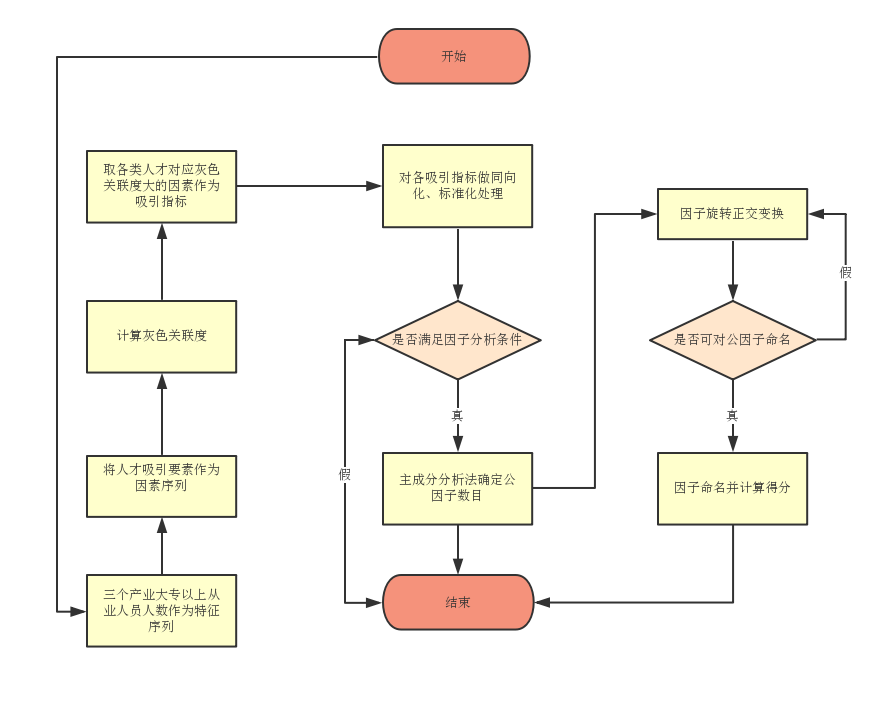
\includegraphics[width=\textwidth]{figures/2222.png}
	\caption{问题二分析流程图}\label{2222}
	\end{figure}



	\subsection{模型的建立与求解}

	\subsubsection{人才及其吸引力影响因素的分类}
	不同产业的人才会有不同的关注焦点,所以城市对不同产业类型的人才吸引力影响因素也存在差异。我们把人才分为三个类型\textbf{——}第一产业人才、第二产业人才和第三产业人才。通过查阅资料\parencite{武汉统计局}收集了武汉2013—2017年第一、第二和第三产业大专以上从业人员人数,所收集数据得到表~\ref{hhh}~如下:
	\begin{table}[H]
		\centering
		\caption{各人才类别从业人数}\label{hhh}
		\begin{tabular}{cccc}
			\toprule[2pt]
			\multicolumn{1}{m{2cm}}{\centering 年份}&
			\multicolumn{1}{m{3cm}}{\centering 第一产业人才} & \multicolumn{1}{m{3cm}}{\centering 第二产业人才} & \multicolumn{1}{m{3cm}}{\centering 第三产业人才}\\
			\midrule[1pt]
			2013	 &  3800 & 1022800&958800\\ 
			2014 & 3571 & 1039720&980144\\ 
			2015	 &  3577&1046760&1022431\\ 
			2016  &  3466& 1053081&1076044\\ 
			2017  & 3229& 1037628&1158174\\
			\bottomrule[2pt]
		\end{tabular}
	\end{table}

	利用灰色关联度理论分别分析三类人才的$33$个影响因素,得到每个影响因子与用电量之间的关联度系数,具体步骤如下:
	确定因素序列和特征序列。本文分别以武汉2013—2017年第一、第二和第三产业大专以上从业人员人数作为特征序列,设为$x_{k}(p)$,采用$n(n=15)$个数据:$x_{k}(p)={x_{k}(1),x_{k}(2),···,x_{k}(5)}(k=1,2,3)$;将$33$个人才吸引要素作为因素序列,设为$x_{i}(t)$,其中有$m(m=33)$个子序列,每个子序列对应$5$个数据:$x_{i}(p)={x_{i}(1),x_{i}(2),···,x_{i}(5)}$。
	
	计算两极最小差 $k$和最大差$K$。计算出特征序列与因素序列的序列差为$\Delta _{i}(t)$,找到结果中的最小差和最大差。其中:
	\begin{gather}
	\begin{array} { l } { \Delta _ { 1 } ( t ) = \left| x _ { 0 } ( t ) - x _ { 1 } ( t ) \right| } \\ { k = \min \min \Delta _ { i } ( t ) } \\ { K = \max \max \Delta _ { i } ( t ) } \end{array}
	\end{gather}
	灰色关联系数和关联度。因素序列和特征序列在第$T$点的关联系数为:
	\begin{gather}
	\Phi _ { 0 , ( p ) } = \frac { k + \varepsilon K } { \Delta _ { 0 i } ( t ) + \varepsilon K }
	\end{gather}
	其中 $\varepsilon$为分辨系数,取$\varepsilon=0.5$。

	利用 MATLAB 软件分析计算后,取各类人才灰色关联度大小前十的影响因素作为其主要影响因素,如表~\ref{guan}~所示:
		\begin{table}[H]
		\centering
		\caption{各人才类别从业人数}\label{guan}
		\begin{tabular}{cccccc}
			\toprule[2pt]
			\multicolumn{1}{m{3cm}}{\centering 第一产业}&
			\multicolumn{1}{m{1.5cm}|}{\centering 关联度} & \multicolumn{1}{m{3cm}}{\centering 第二产业} & \multicolumn{1}{m{1.5cm}|}{\centering 关联度}&
			\multicolumn{1}{m{3cm}}{\centering 第三产业} & \multicolumn{1}{m{1.5cm}}{\centering 关联度}\\
			\midrule[1pt]
			经济增长率	 &  0.897 & 农业&0.862&第三产业占比&0.978\\ 
			旅游业 &  0.874&第二产业&0.807&邮政业&0.958\\ 
			第三产业占比	 &  0.840&客运量(万人)&0.787&旅游业&0.933\\ 
			固定资产总额&  0.827& 商品房销售价格&0.771&年末电话用户&0.925\\ 
			房地产和投资业  & 0.786& 工业和建筑业&0.756&剧场、影剧院&0.922\\
			职工平均工资  &0.728& 执业/助理医师&0.748&地区生产总值&0.921\\
			人均GDP(元/人)  & 0.719& 固定资产总额&0.742&年末邮政局数&0.915\\
			在岗职工平均工资  & 0.711& 年末邮政局数&0.737&固定资产总额&0.907\\
			地方财政内收入  & 0.643& 地方财政内支出&0.736&货运量(万吨)&0.902\\
			地方财政内支出&0.643& 邮政业&0.726&客运量(万人)&0.887\\
			地区生产总值&0.615&消费品零售总额&0.716&地方财政内收入&0.880\\
			\bottomrule[2pt]
		\end{tabular}
	\end{table}
	
	
	\subsubsection{分类型人才吸引力分析}
	将归类后所得的影响第一产业人才吸引力的$10$个影响因素在五个城市中2013—2017年的数据,使用SPSS进行因子分析,按照累积贡献率的原则提取公因子,以综合性指标来相对全面的反映出全体因子对第一产业人才吸引力的影响情况。按照主因子的提取原则,通过碎石图可看出可以用$3$个主因子来描述此$10$个因子的影响;再通过旋转后因子贡献率计算所得的城市各因子得分得到各城市每年的第一产业人才吸引力综合得分。其计算公式如下:
	\begin{gather}
	\mathrm { F } = \left( 48.328 \mathrm { F } _ { 1 } + 28.667 \mathrm { F } _ { 2 } + 12.283 \mathrm { F } _ { 3 } \right) / 89.277
	%(附结果计算公式)
	\end{gather}
	将得到的五个城市2013—2017年的综合得分绘制为折线图的到图~\ref{11}~如下所示:
	\begin{figure}[H]
		\centering
		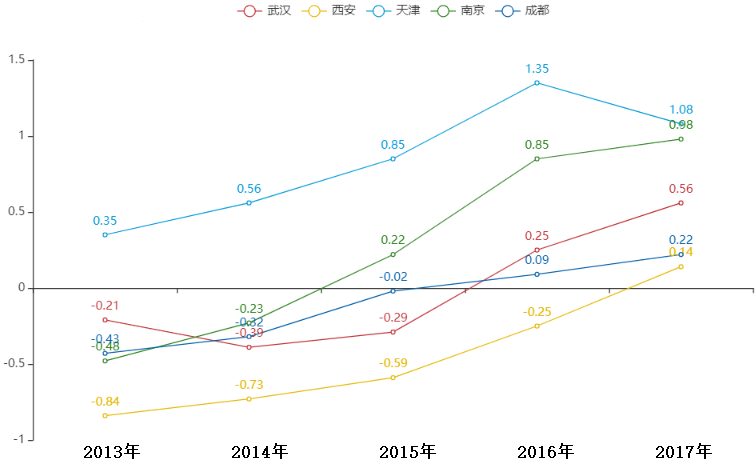
\includegraphics[width=.9\textwidth]{figures/11.png}
		\caption{第一产业人才吸引力综合得分折线图}\label{11}
	\end{figure} 
	同理将归类后所得的影响第二产业人才吸引力的$10$个影响因素使用SPSS进行因子分析,得到第二产业人才吸引力综合得分计算公式:
	\begin{gather}
	\mathrm { F } = \left( 27.594 \mathrm { F } _ { 1 } + 26.960 \mathrm { F } _ { 2 } + 16.609 \mathrm { F } _ { 3 } + 16.356 \mathrm { F } _ { 4 } \right) / 87.519
	%(附结果计算公式)
	\end{gather}
	第二产业人才吸引力综合得分折线图:
	\begin{figure}[H]
		\centering
		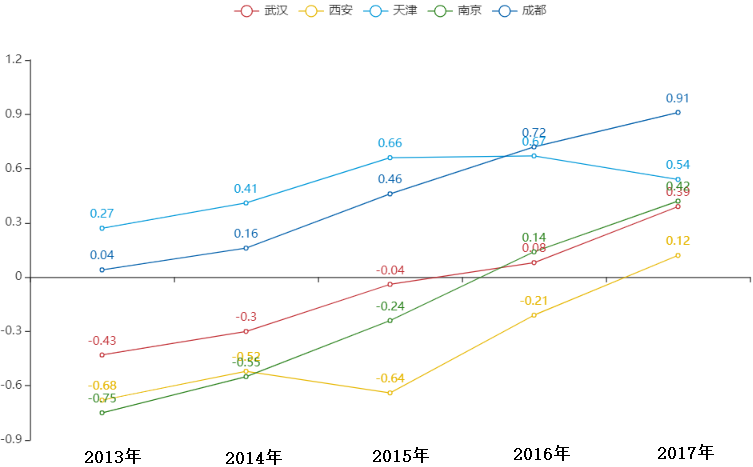
\includegraphics[width=.9\textwidth]{figures/22.png}
		\caption{第二产业人才吸引力综合得分折线图}\label{22}
	\end{figure}
	
	同理将归类后所得的影响第三产业人才吸引力的$10$个影响因素使用SPSS进行因子分析,得到第二产业人才吸引力综合得分计算公式:
	\begin{gather}
	\mathrm { F } = \left( 37.063 \mathrm { F } _ { 1 } + 25.130 \mathrm { F } _ { 2 } + 11.972 \mathrm { F } _ { 3 } + 10.477 \mathrm { F } _ { 4 } \right) / 84.642
	%(附结果计算公式)
	\end{gather}

	第三产业人才吸引力综合得分折线图:
		\begin{figure}[H]
		\centering
		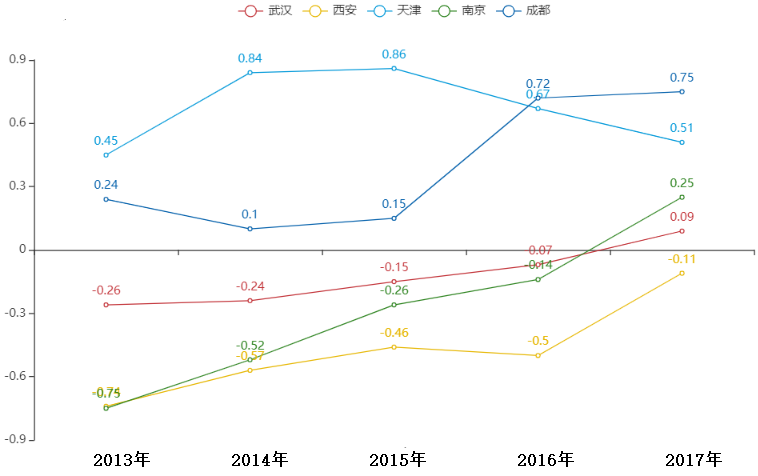
\includegraphics[width=\textwidth]{figures/33.png}
		\caption{第三产业人才吸引力综合得分折线图}\label{33}
	\end{figure}


	\subsection{结果分析}
	由图表可以看出,武汉市的人才吸引力水平近几年有较高的水平,尤其是对第二、三产业人才的吸引力表现出逐年增加趋势和较高水平,相对于西安和成都而言,武汉市具有较强的人才吸引力,十分符合地区的经
	济发展特点。而天津作为老牌北方直辖市,近年发展速度相比略显缓慢,导致其相应人才吸引力也有所下滑。
	
	但是,武汉在发展中也存在一些不足。特别是工业发展与薪酬因子处于人才吸引主导地位,而环境方面的因素尚未
	完全建立;优质教育与医疗资源分
	配不均、生活成本高、高校科研机构偏少等因素限制良好人才环境
	构建等。
	
	提高武汉市的人才吸引力水平,提出以下几点建议:
\begin{itemize}
	\item [(1)] 大力发展地方生产总值,为经济社会发展打下坚实的基础。
	\item [(2)]主要行业是加快人
	才发展的主导力量。建立较为高效的人才市场,通过各行业市场
	机制,人才较为充分地实现了自身价值,也为武汉的人才持续发展创
	造了良好条件。
	\item [(3)]注重整合空间结构全面发展,引导各大区块均衡协调稳步发展,
	建设全面型社会,注重生态建设,贯彻落实以人为本的科学发展理
	念。
	\item [(4)]加大营商环境改革力度,营
	造更加开放的贸易投资环境,营造综合成本适宜的产业发展环境,
	营造更加高效透明的政务环境。
	\item [(5)]政府不断完善就业服务政策,出台大量相关文件,高度重视高
	校毕业生的就业情况。
\end{itemize}

	\section{写给武汉市人力资源部门的建议报告}
	

	\paragraph{武汉市人力资源管理部分的领导您好:}
	~\\
	
	武汉市作为全国科技和教育事业最发达的地区之一, 无论在拥有高校数量还是毕业生质量方面都位居前列。就业政策体系不断完善,扶持就业创业力度不断加大,社会保障体系建设取得突破性进展,人才队伍建设卓有成效。随着”黄鹤英才计划”,”3551人才计划”等重大人才工程的推进,累计引进,培养中央”千人计划”、国家”万人计划”、省”百人计划”等顶尖人才375人,吸纳引进海内外高层次创新创业人才4000余人,数量居中部城市第一。
	
	人才决定着一个城市的发展前景, 但城市必须拥有足够的吸引力才能让人才流入。人才在选择移居城市时必然会去对这个城市进行量化评估并与其他城市进行对比, 进而去选择最适和发展的城市。发展前景,迁移成本、薪资待遇以及城市各方面环境因素、政府策略都是会是考虑的因素。我们只有紧紧抓住人才这个关键环节,才能在新一轮经济发展和城市竞争中取得优势,因此我们建立了人才吸引力影响因素和政策效力的模型,在政策制定有很大的理论和现实意义,并向贵部门提出相关建议。
	
	通过2013-2017年国家统计年鉴和每年各大城市统计年鉴和各式人力资源和社会保障局官网的相关数据为依据,对以武汉市在内的同类型城市(西安、成都、天津、南京、武汉)人才吸引力水平进行分析。我们结合了因子分析法和主成分分析法地代数模型进行研究,首先构建评价指标体系。遵循客观地、科学性和系统性地原则选取了城市发展前景、主要行业收入、政府影响、环境因素、年末总人口共5个二级指标和33个三级指标。并应用因子分析将33个三级指标综合成4个公共因子,这4个公因子的累计方差达到$99.2\%$。用这4个公因子来对武汉城市吸引力进行评价,再利用主成分分析法提取,构建未转轴的因子载荷矩阵,得到因子的分析模型后,进行正交旋转,对两级分化的因子系数进行命名,第一个主因子包含地区生产总值、第一第二产业生产总值、在岗职工平均工资和人均GDP等,这些指标包含了地区工业发展水平以及人均薪酬水平故将其命名为\textbf{工业发展与薪酬因子},第二个主因子包含持证医师人数,医院卫生院个数以及一年内空气质量达到及好于二级的天数等,这些指标包含了地区医疗卫生水平和居民生活环境,故将其命名为\textbf{医疗卫生环境因子},第三个主因子包含固定资产投资总额与货物进出口总额,该指标反映了城市贸易与经济发展水平,故将其命名为\textbf{经济贸易因子},第四个主因子包含年末总人口与旅游生产总值,反映了城市人口与拥挤程度故将其命名人口与\textbf{拥挤程度因子}。多次旋转迭代后的成分矩阵已收敛,得到最终的人才吸引力评价模型,计算各因子的作用权重,并给出武汉城市的综合因子得分。研究数据表明影响人才吸引力最主要因素是工业发展与薪酬,其次是医疗卫生环境因子,再者是经济贸易因子,最后是拥挤程度因子。从中可以看出,吸引人才的首先是一个地区发展前景和薪资水平的高低,,虽然地区交通拥挤程度也很重要,但对于个人而言,医疗卫生环境和经济贸易发展更为关键。
	
	因此,针对以上情况我们向有关领导提出以下建议:
	\begin{itemize}
		\item [(1)] 促进城市经济发展,增加城市提供就业机会能力, 大力实施大众创业万众创新战略,着力打造创业梦想之城。人才被城市的经济发展水平及其提供的发展前景所吸引。发展经济是吸引人才的基础条件, 要从区域、产业、企业三个层次促进经济的发展.依靠核心城市群的带动作用, 加强区域协调发展,统筹城乡就业工作, 推动生产要素在区域内自由流和优化配置.解决结构性就业矛盾,把产业规划和人才引进规划匹配起来。企业作为吸纳人才的主体, 要为企业的发展提供宽松稳定的环境与高效清明的服务环境, 对企业实行税收上的减免与政策上的扶持, 增强企业的实力及其对人才的吸引能力。
		\item [(2)]改善公共服务与自然环境, 加强城市舒适性建设.从满足不同层次需求的角度来说, 高层次的需求是在经济水平之上的更加舒适的生活环境.加强城市规划、加快基本公共服务供给侧结构改革。建立更加公平可持续的社会保障制度,着力构建社会和谐之基。进一步推进社会保障制度改革,建立健全社会保障待遇确定和正常调整机制。建立健全社会保险市级统筹制度,完善筹资机制。继续做好社会保险扩面工作,要以人为本,促进社会和谐发展,增强城市对于生活质量要求较高人才的吸引力。
		\item [(3)]优化城市人才政策, 增强城市为人才提供就业服务的能力。着力于打造国际性创行人才高地。不断优化人才创新创业环境,创新工作体制机制。积极打造国际人才自由港,努力组建规模宏大、具有较强国际竞争力、引领支撑国家创新中心建设的人才队伍。发挥市场调节供需关系的作用.充分尊重人才的成长规律, 人才的评价与激励涵盖人才的品德等方面, 同时尊重市场的规律, 实现人才资源的最优组合.更注重对人才的人文关怀和人才个人价值体现, 从而体现以人为本的发展理念。
		建设全面型社会,注重生态建设,贯彻落实以人为本的科学发展理
		念。
	\end{itemize}


	总之,一切
	政策都是为了发展,人才就是发展的基础。紧抓落实人才政策,实施人才战略才符合良好人才环境的营造。此次研究还存在一些局限性,受采集数据的限制,与现实情况之间出现一些偏差。以上建议供领导参考,不足之处请予以批评指正。



	\section{模型的评价}
	\subsection{模型的优点}
	\begin{itemize}
		\item [(1)] 从国家统计数据库、武汉市统计年鉴和其他同类城市的统计年鉴中爬取大量数据,并挑选符合实际的33个指标与最近五年的数据进行评价。其吸引人才指标从多维度、全方面的考虑,具备科学性、客观性。
		\item [(2)]针对具体人才根据相应产业进行分类。相较于现有城市人才吸引力水平评价模型,我们采用了灰色关联分析法,对三种人才类别分析计算出与指标的相关系数,求出不同人才对33种影响因素的的偏好程度,选出前十个合适的指标进行综合打分。
	\end{itemize}

	
	\subsection{模型的缺点}
    未能具体地量化政府政策对人口吸引力的影响,只选取了地方财政收入、支出,固定资产投资总额三个影响因素作为政策影响的指标,与现实情况出现一定偏差,存在一定的局限性。

    
    
	\newpage	%换页符
	%%参考文献
	%\begin{thebibliography}{9}%宽度9
	% \setlength{\itemsep}{-2mm}
	\nocite{*}		%排版未引用的参考文献
	\printbibliography[title = {参考文献}]	%使用国标参考文献添加方式
	%参考文献添加到wenxian.bib里,再引用
	
	\newpage
	%附录
	\appendix %%附录
\section{代码}
\subsection{数据预处理--python源代码}
\begin{lstlisting}[language=python]%这里修改语言
import pandas as pd
from sklearn.preprocessing import StandardScaler
from sklearn.decomposition import PCA
from factor_analyzer import FactorAnalyzer

#导入数据
df = pd.read_excel("wut.xls")
# print(df.head(5))

#转置
df = pd.DataFrame(df.values.T, index=df.columns, columns=df.index)
# print(df['商品房平均销售价格(元/平方米)'])

数据正向处理
df['商品房平均销售价格(元/平方米)'] = -(df['商品房平均销售价格(元/平方米)']-sum(df['商品房平均销售价格(元/平方米)'])/5)
df['工业废水排放量(万吨)'] = -(df['工业废水排放量(万吨)']-sum(df['工业废水排放量(万吨)'])/5)
df['工业二氧化硫排放量(吨)'] = -(df['工业二氧化硫排放量(吨)']-sum(df['工业二氧化硫排放量(吨)'])/5)
print(df['商品房平均销售价格(元/平方米)'])
print(df.head(5))
df.to_excel("武汉.xls")

#数据标准化
df = StandardScaler().fit_transform(df)
# print(df)
df=pd.DataFrame(df)
df.to_excel("武汉.xls")
#
#主成分分析
pca = PCA(n_components=4)
newX = pca.fit_transform(df)
print(newX)

#返回所保留的n个成分各自的方差百分比
print("它代表降维后的各主成分的方差值占总方差值的比例,这个比例越大,则越是重要的主成分")
print(pca.explained_variance_ratio_)
print("它代表降维后的各主成分的方差值,方差值越大,则说明越是重要的主成分")
print(pca.explained_variance_)

\end{lstlisting}
\subsection{数据可视化--python源代码}
\begin{lstlisting}[language=python]%这里修改语言
from example.commons import Faker
from pyecharts import options as opts
from pyecharts.charts import Bar
from pyecharts.globals import ThemeType


def bar_xyaxis_name() -> Bar:
c = (
Bar(init_opts=opts.InitOpts(theme=ThemeType.WHITE))
.add_xaxis(['2013年','2014年','2015年','2016年','2017年'])
.add_yaxis("得分",[-77.99,-30.08,-11.90,42.35,77.63])
.set_global_opts(
title_opts=opts.TitleOpts(title="综合因子得分"),
# yaxis_opts=opts.AxisOpts(name="Score"),
toolbox_opts=opts.ToolboxOpts(),
# xaxis_opts=opts.AxisOpts(name="Year"),

brush_opts=opts.BrushOpts(),
)
# .add(is_datazoom_show=True)
)
return c


b = bar_xyaxis_name()
b.render()
\end{lstlisting}
\subsection{灰色关联度--matlab源代码}
\begin{lstlisting}
clear;
clc;
a=xlsread('wh.xls','B2:AH6');
[m,n]=size(a);
cankao=xlsread('sanchanb.xls','D2:D6');%参考矩阵输入
t=repmat(cankao,[1,n])-a;%求参考序列与每一个序列的差
mmin=min(min(t));%计算最小差
mmax=max(max(t));%计算最大差
rho=0.5;%分辨系数
xishu=(mmin+rho*mmax)./(t+rho*mmax);%计算灰色关联系数
guanliandu=mean(xishu);%取等权重,计算关联度
[gsort,ind]=sort(guanliandu,'descend');%对关联度排序
\end{lstlisting}
\subsection{相关系数矩阵}
\begin{table}
	\centering
	\caption{相关系数矩阵}
	\begin{tabular}{|l|l|l|l|l|l|l|l|l|l|l|l|l|l|l|l|l|l|l|l|l|l|l|l|l|l|l|l|l|l|l|l|l|}
		\hline
		
		1.000 & 0.727 & -0.423 & 0.967 & 0.973 & 0.937 & 0.799 & 0.989 & 0.989 & -0.988 & 0.994 & 0.969 & 0.960 & 0.797 & 0.898 & 0.246 & -0.670 & -0.898 & 0.614 & -0.119 & 0.914 & -0.927 & 0.985 & 0.991 & 0.513 & 0.766 & 0.967 & -0.963 & 0.984 & 0.954 & 0.973 & 0.881 & -0.928 \\ \hline
		0.727 & 1.000 & -0.796 & 0.822 & 0.832 & 0.721 & 0.760 & 0.707 & 0.802 & -0.657 & 0.716 & 0.746 & 0.785 & 0.318 & 0.465 & -0.478 & -0.615 & -0.674 & 0.436 & -0.603 & 0.422 & -0.690 & 0.813 & 0.793 & 0.930 & 0.762 & 0.699 & -0.737 & 0.814 & 0.582 & 0.816 & 0.881 & -0.814 \\ \hline
		-0.423 & -0.796 & 1.000 & -0.620 & -0.470 & -0.293 & -0.825 & -0.469 & -0.518 & 0.311 & -0.357 & -0.586 & -0.629 & 0.034 & -0.179 & 0.493 & 0.016 & 0.164 & -0.428 & 0.873 & -0.213 & 0.597 & -0.569 & -0.529 & -0.674 & -0.758 & -0.534 & 0.593 & -0.561 & -0.424 & -0.493 & -0.689 & 0.682 \\ \hline
		0.967 & 0.822 & -0.620 & 1.000 & 0.947 & 0.853 & 0.909 & 0.961 & 0.973 & -0.919 & 0.941 & 0.985 & 0.996 & 0.720 & 0.854 & 0.094 & -0.578 & -0.797 & 0.713 & -0.285 & 0.831 & -0.970 & 0.995 & 0.982 & 0.585 & 0.895 & 0.981 & -0.985 & 0.980 & 0.927 & 0.944 & 0.961 & -0.955 \\ \hline
		0.973 & 0.832 & -0.470 & 0.947 & 1.000 & 0.969 & 0.752 & 0.951 & 0.986 & -0.961 & 0.981 & 0.925 & 0.922 & 0.704 & 0.806 & 0.048 & -0.771 & -0.940 & 0.512 & -0.211 & 0.816 & -0.854 & 0.971 & 0.979 & 0.685 & 0.726 & 0.905 & -0.912 & 0.978 & 0.872 & 0.992 & 0.889 & -0.918 \\ \hline
		0.937 & 0.721 & -0.293 & 0.853 & 0.969 & 1.000 & 0.608 & 0.919 & 0.947 & -0.962 & 0.965 & 0.851 & 0.827 & 0.671 & 0.750 & 0.142 & -0.801 & -0.978 & 0.326 & -0.114 & 0.832 & -0.745 & 0.899 & 0.930 & 0.624 & 0.540 & 0.822 & -0.830 & 0.928 & 0.835 & 0.971 & 0.748 & -0.855 \\ \hline
		0.799 & 0.760 & -0.825 & 0.909 & 0.752 & 0.608 & 1.000 & 0.838 & 0.828 & -0.718 & 0.735 & 0.917 & 0.933 & 0.473 & 0.665 & 0.025 & -0.208 & -0.489 & 0.712 & -0.537 & 0.702 & -0.939 & 0.876 & 0.849 & 0.493 & 0.933 & 0.903 & -0.926 & 0.858 & 0.846 & 0.777 & 0.881 & -0.919 \\ \hline
		0.989 & 0.707 & -0.469 & 0.961 & 0.951 & 0.919 & 0.838 & 1.000 & 0.987 & -0.979 & 0.976 & 0.985 & 0.965 & 0.731 & 0.858 & 0.279 & -0.570 & -0.850 & 0.573 & -0.201 & 0.939 & -0.937 & 0.978 & 0.990 & 0.486 & 0.757 & 0.972 & -0.977 & 0.986 & 0.979 & 0.969 & 0.850 & -0.960 \\ \hline
		0.989 & 0.802 & -0.518 & 0.973 & 0.986 & 0.947 & 0.828 & 0.987 & 1.000 & -0.973 & 0.982 & 0.972 & 0.963 & 0.700 & 0.826 & 0.134 & -0.659 & -0.891 & 0.551 & -0.254 & 0.876 & -0.913 & 0.990 & 0.999 & 0.615 & 0.769 & 0.952 & -0.962 & 0.998 & 0.935 & 0.993 & 0.891 & -0.963 \\ \hline
		-0.988 & -0.657 & 0.311 & -0.919 & -0.961 & -0.962 & -0.718 & -0.979 & -0.973 & 1.000 & -0.995 & -0.935 & -0.911 & -0.794 & -0.881 & -0.321 & 0.691 & 0.928 & -0.515 & 0.048 & -0.938 & 0.872 & -0.950 & -0.970 & -0.467 & -0.662 & -0.929 & 0.924 & -0.961 & -0.945 & -0.967 & -0.802 & 0.896 \\ \hline
		0.994 & 0.716 & -0.357 & 0.941 & 0.981 & 0.965 & 0.735 & 0.976 & 0.982 & -0.995 & 1.000 & 0.940 & 0.926 & 0.798 & 0.885 & 0.241 & -0.732 & -0.939 & 0.553 & -0.073 & 0.904 & -0.882 & 0.967 & 0.980 & 0.529 & 0.705 & 0.935 & -0.930 & 0.972 & 0.928 & 0.977 & 0.850 & -0.901 \\ \hline
		0.969 & 0.746 & -0.586 & 0.985 & 0.925 & 0.851 & 0.917 & 0.985 & 0.972 & -0.935 & 0.940 & 1.000 & 0.994 & 0.705 & 0.851 & 0.217 & -0.491 & -0.772 & 0.668 & -0.283 & 0.899 & -0.979 & 0.985 & 0.982 & 0.495 & 0.854 & 0.992 & -0.999 & 0.981 & 0.973 & 0.940 & 0.902 & -0.974 \\ \hline
		0.960 & 0.785 & -0.629 & 0.996 & 0.922 & 0.827 & 0.933 & 0.965 & 0.963 & -0.911 & 0.926 & 0.994 & 1.000 & 0.709 & 0.853 & 0.148 & -0.505 & -0.756 & 0.722 & -0.298 & 0.854 & -0.986 & 0.988 & 0.975 & 0.530 & 0.901 & 0.991 & -0.996 & 0.974 & 0.948 & 0.928 & 0.942 & -0.963 \\ \hline
		0.797 & 0.318 & 0.034 & 0.720 & 0.704 & 0.671 & 0.473 & 0.731 & 0.700 & -0.794 & 0.798 & 0.705 & 0.709 & 1.000 & 0.971 & 0.522 & -0.632 & -0.733 & 0.751 & 0.456 & 0.776 & -0.742 & 0.730 & 0.717 & 0.062 & 0.604 & 0.777 & -0.715 & 0.681 & 0.754 & 0.656 & 0.675 & -0.539 \\ \hline
		0.898 & 0.465 & -0.179 & 0.854 & 0.806 & 0.750 & 0.665 & 0.858 & 0.826 & -0.881 & 0.885 & 0.851 & 0.853 & 0.971 & 1.000 & 0.473 & -0.591 & -0.766 & 0.800 & 0.241 & 0.868 & -0.880 & 0.857 & 0.844 & 0.180 & 0.743 & 0.904 & -0.860 & 0.817 & 0.880 & 0.777 & 0.795 & -0.714 \\ \hline
		0.246 & -0.478 & 0.493 & 0.094 & 0.048 & 0.142 & 0.025 & 0.279 & 0.134 & -0.321 & 0.241 & 0.217 & 0.148 & 0.522 & 0.473 & 1.000 & 0.122 & -0.131 & 0.196 & 0.606 & 0.588 & -0.252 & 0.120 & 0.154 & -0.679 & -0.047 & 0.277 & -0.224 & 0.118 & 0.429 & 0.084 & -0.108 & -0.077 \\ \hline
		-0.670 & -0.615 & 0.016 & -0.578 & -0.771 & -0.801 & -0.208 & -0.570 & -0.659 & 0.691 & -0.732 & -0.491 & -0.505 & -0.632 & -0.591 & 0.122 & 1.000 & 0.900 & -0.247 & -0.182 & -0.433 & 0.402 & -0.624 & -0.635 & -0.632 & -0.325 & -0.492 & 0.472 & -0.624 & -0.430 & -0.706 & -0.598 & 0.459 \\ \hline
		-0.898 & -0.674 & 0.164 & -0.797 & -0.940 & -0.978 & -0.489 & -0.850 & -0.891 & 0.928 & -0.939 & -0.772 & -0.756 & -0.733 & -0.766 & -0.131 & 0.900 & 1.000 & -0.336 & -0.044 & -0.766 & 0.673 & -0.846 & -0.873 & -0.597 & -0.485 & -0.759 & 0.752 & -0.864 & -0.755 & -0.920 & -0.720 & 0.750 \\ \hline
		0.614 & 0.436 & -0.428 & 0.713 & 0.512 & 0.326 & 0.712 & 0.573 & 0.551 & -0.515 & 0.553 & 0.668 & 0.722 & 0.751 & 0.800 & 0.196 & -0.247 & -0.336 & 1.000 & 0.060 & 0.510 & -0.797 & 0.657 & 0.591 & 0.105 & 0.887 & 0.744 & -0.700 & 0.569 & 0.625 & 0.463 & 0.786 & -0.521 \\ \hline
		-0.119 & -0.603 & 0.873 & -0.285 & -0.211 & -0.114 & -0.537 & -0.201 & -0.254 & 0.048 & -0.073 & -0.283 & -0.298 & 0.456 & 0.241 & 0.606 & -0.182 & -0.044 & 0.060 & 1.000 & 0.031 & 0.233 & -0.257 & -0.248 & -0.632 & -0.356 & -0.186 & 0.274 & -0.295 & -0.137 & -0.269 & -0.313 & 0.465 \\ \hline
		0.914 & 0.422 & -0.213 & 0.831 & 0.816 & 0.832 & 0.702 & 0.939 & 0.876 & -0.938 & 0.904 & 0.899 & 0.854 & 0.776 & 0.868 & 0.588 & -0.433 & -0.766 & 0.510 & 0.031 & 1.000 & -0.862 & 0.858 & 0.884 & 0.176 & 0.593 & 0.904 & -0.893 & 0.870 & 0.972 & 0.848 & 0.656 & -0.837 \\ \hline
		-0.927 & -0.690 & 0.597 & -0.970 & -0.854 & -0.745 & -0.939 & -0.937 & -0.913 & 0.872 & -0.882 & -0.979 & -0.986 & -0.742 & -0.880 & -0.252 & 0.402 & 0.673 & -0.797 & 0.233 & -0.862 & 1.000 & -0.953 & -0.934 & -0.392 & -0.919 & -0.991 & 0.988 & -0.927 & -0.953 & -0.861 & -0.914 & 0.921 \\ \hline
		0.985 & 0.813 & -0.569 & 0.995 & 0.971 & 0.899 & 0.876 & 0.978 & 0.990 & -0.950 & 0.967 & 0.985 & 0.988 & 0.730 & 0.857 & 0.120 & -0.624 & -0.846 & 0.657 & -0.257 & 0.858 & -0.953 & 1.000 & 0.995 & 0.594 & 0.848 & 0.977 & -0.982 & 0.993 & 0.937 & 0.970 & 0.939 & -0.960 \\ \hline
		0.991 & 0.793 & -0.529 & 0.982 & 0.979 & 0.930 & 0.849 & 0.990 & 0.999 & -0.970 & 0.980 & 0.982 & 0.975 & 0.717 & 0.844 & 0.154 & -0.635 & -0.873 & 0.591 & -0.248 & 0.884 & -0.934 & 0.995 & 1.000 & 0.589 & 0.796 & 0.967 & -0.975 & 0.999 & 0.947 & 0.986 & 0.903 & -0.966 \\ \hline
		0.513 & 0.930 & -0.674 & 0.585 & 0.685 & 0.624 & 0.493 & 0.486 & 0.615 & -0.467 & 0.529 & 0.495 & 0.530 & 0.062 & 0.180 & -0.679 & -0.632 & -0.597 & 0.105 & -0.632 & 0.176 & -0.392 & 0.594 & 0.589 & 1.000 & 0.477 & 0.422 & -0.475 & 0.619 & 0.314 & 0.667 & 0.659 & -0.617 \\ \hline
		0.766 & 0.762 & -0.758 & 0.895 & 0.726 & 0.540 & 0.933 & 0.757 & 0.769 & -0.662 & 0.705 & 0.854 & 0.901 & 0.604 & 0.743 & -0.047 & -0.325 & -0.485 & 0.887 & -0.356 & 0.593 & -0.919 & 0.848 & 0.796 & 0.477 & 1.000 & 0.874 & -0.873 & 0.795 & 0.756 & 0.707 & 0.947 & -0.802 \\ \hline
		0.967 & 0.699 & -0.534 & 0.981 & 0.905 & 0.822 & 0.903 & 0.972 & 0.952 & -0.929 & 0.935 & 0.992 & 0.991 & 0.777 & 0.904 & 0.277 & -0.492 & -0.759 & 0.744 & -0.186 & 0.904 & -0.991 & 0.977 & 0.967 & 0.422 & 0.874 & 1.000 & -0.995 & 0.960 & 0.974 & 0.911 & 0.908 & -0.937 \\ \hline
		-0.963 & -0.737 & 0.593 & -0.985 & -0.912 & -0.830 & -0.926 & -0.977 & -0.962 & 0.924 & -0.930 & -0.999 & -0.996 & -0.715 & -0.860 & -0.224 & 0.472 & 0.752 & -0.700 & 0.274 & -0.893 & 0.988 & -0.982 & -0.975 & -0.475 & -0.873 & -0.995 & 1.000 & -0.972 & -0.972 & -0.926 & -0.909 & 0.966 \\ \hline
		0.984 & 0.814 & -0.561 & 0.980 & 0.978 & 0.928 & 0.858 & 0.986 & 0.998 & -0.961 & 0.972 & 0.981 & 0.974 & 0.681 & 0.817 & 0.118 & -0.624 & -0.864 & 0.569 & -0.295 & 0.870 & -0.927 & 0.993 & 0.999 & 0.619 & 0.795 & 0.960 & -0.972 & 1.000 & 0.938 & 0.988 & 0.903 & -0.975 \\ \hline
		0.954 & 0.582 & -0.424 & 0.927 & 0.872 & 0.835 & 0.846 & 0.979 & 0.935 & -0.945 & 0.928 & 0.973 & 0.948 & 0.754 & 0.880 & 0.429 & -0.430 & -0.755 & 0.625 & -0.137 & 0.972 & -0.953 & 0.937 & 0.947 & 0.314 & 0.756 & 0.974 & -0.972 & 0.938 & 1.000 & 0.898 & 0.796 & -0.925 \\ \hline
		0.973 & 0.816 & -0.493 & 0.944 & 0.992 & 0.971 & 0.777 & 0.969 & 0.993 & -0.967 & 0.977 & 0.940 & 0.928 & 0.656 & 0.777 & 0.084 & -0.706 & -0.920 & 0.463 & -0.269 & 0.848 & -0.861 & 0.970 & 0.986 & 0.667 & 0.707 & 0.911 & -0.926 & 0.988 & 0.898 & 1.000 & 0.860 & -0.949 \\ \hline
		0.881 & 0.881 & -0.689 & 0.961 & 0.889 & 0.748 & 0.881 & 0.850 & 0.891 & -0.802 & 0.850 & 0.902 & 0.942 & 0.675 & 0.795 & -0.108 & -0.598 & -0.720 & 0.786 & -0.313 & 0.656 & -0.914 & 0.939 & 0.903 & 0.659 & 0.947 & 0.908 & -0.909 & 0.903 & 0.796 & 0.860 & 1.000 & -0.867 \\ \hline
		-0.928 & -0.814 & 0.682 & -0.955 & -0.918 & -0.855 & -0.919 & -0.960 & -0.963 & 0.896 & -0.901 & -0.974 & -0.963 & -0.539 & -0.714 & -0.077 & 0.459 & 0.750 & -0.521 & 0.465 & -0.837 & 0.921 & -0.960 & -0.966 & -0.617 & -0.802 & -0.937 & 0.966 & -0.975 & -0.925 & -0.949 & -0.867 & 1.000 \\ \hline
		
	\end{tabular}
\end{table}
\subsection{初始因子载荷矩阵}
	\begin{figure}[H]
	\centering
	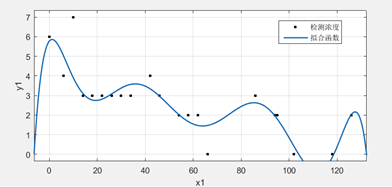
\includegraphics[width=\textwidth]{figures/1.png}

\end{figure}  

	\begin{figure}[H]
	\centering
	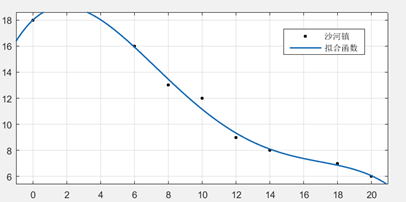
\includegraphics[width=\textwidth]{figures/2.png}

\end{figure} 
\subsection{旋转后的因子载荷矩阵}
\begin{figure}[H]
	\centering
	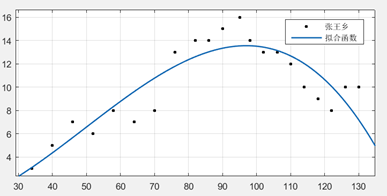
\includegraphics[width=\textwidth]{figures/3.png}
	
\end{figure}  

\begin{figure}[H]
	\centering
	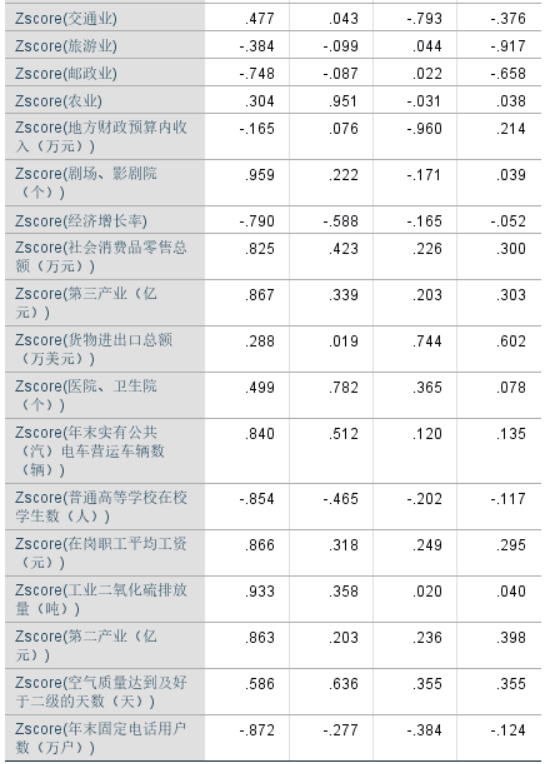
\includegraphics[width=\textwidth]{figures/4.png}
	
\end{figure}
\subsection{成分得分系数矩阵}
\begin{figure}[H]
	\centering
	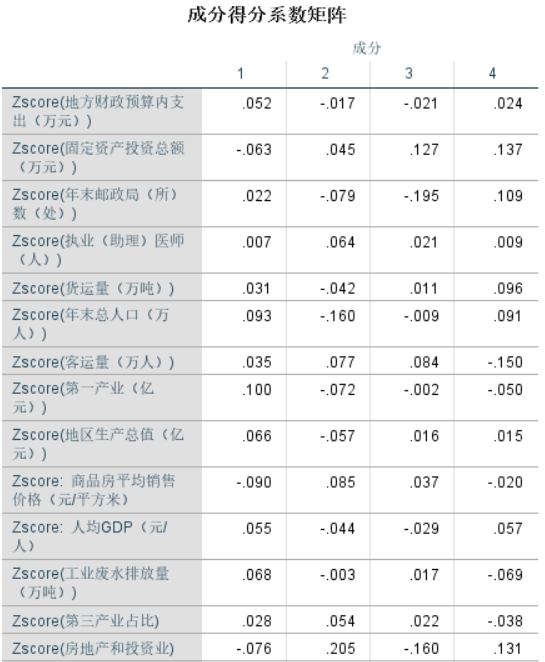
\includegraphics[width=\textwidth]{figures/5.png}
	
\end{figure}  

\begin{figure}[H]
	\centering
	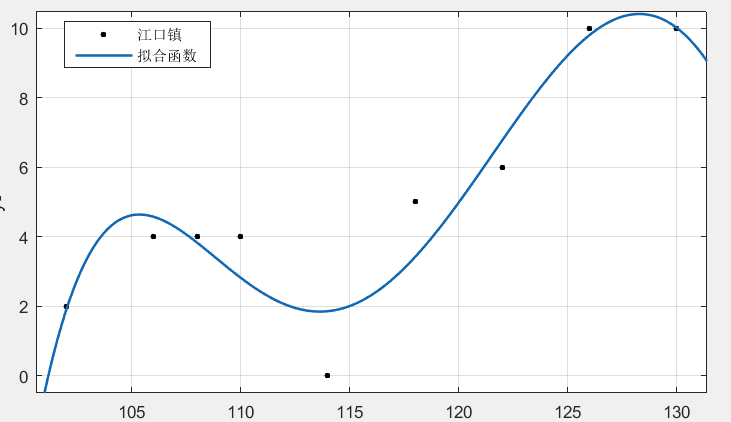
\includegraphics[width=\textwidth]{figures/6.png}
	
\end{figure}

\end{document}